% Integral de línea: dr tangente al camino C (libro fig. 2.2)
\documentclass[border=4pt]{standalone}
\usepackage{tikz}
\usetikzlibrary{arrows.meta, calc}
\begin{document}
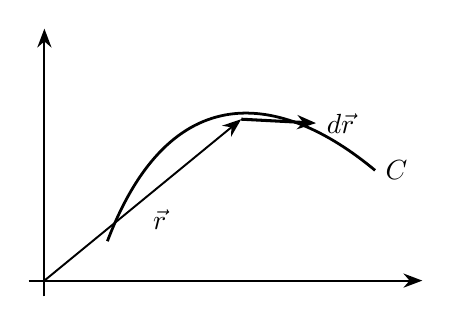
\begin{tikzpicture}[>={Stealth[length=2.4mm]}, line width=0.7pt]
  \draw[->] (-0.2,0)--(4.8,0);
  \draw[->] (0,-0.2)--(0,3.2);
  \draw[line width=1pt] (0.8,0.5) .. controls (1.6,2.6) and (3.0,2.4) .. (4.2,1.4) node[right]{$C$};
  \coordinate (P) at (2.5,2.05);
  \draw[->] (0,0)--(P) node[midway, below right]{$\vec r$};
  \draw[->, line width=1.1pt] (P)--($(P)+(0.95,-0.05)$) node[right]{$d\vec r$};
\end{tikzpicture}
\end{document}
